Chapter 6

\chapter{Tools} % Main chapter title

\label{Chapter6} % For referencing the chapter elsewhere, use \ref{Chapter1} 

\lhead{Chapter 6. \emph{Tools}} % This is for the header on each page - perhaps a shortened title

%----------------------------------------------------------------------------------------

\section{AWN}
Arabic WordNet is the Arabic analogue to the widely used WordNet for the English language. The Arabic WordNet (AWN) is a lexical database of the Arabic language following the development process of Princeton English WordNet and Euro WordNet. It utilizes the Suggested Upper Merged Ontology as an interlingua to link Arabic WordNet to previously developed wordnets. Christiane Fellbaum at Princeton was the project lead. The project was sponsored by DOI/REFLEX.\\
From http://www.globalwordnet.org/AWN/DataSpec.html you can get the XML data exchange specifications of the database. AWN contains about 11,000 synsets (including 1,000 NE).\\

There are several different ways for accessing the database:\\
\begin{itemize}
\item[1] The browser package (available at http://sourceforge.net/projects/awnbrowser/) includes the AWN data and Princeton WN2.0 mappings in a relational database. You can use the export facilities to export the data as XML or CSV to taylor them to your needs .\\
\item[2] The database can also be downloaded in XML format (linked to Princeton WN 2.0) from \url {http://nlp.lsi.upc.edu/awn/get_bd.php}\\
\item[3] A set of basic python functions for accessing the database can be obtained from: \url {http://nlp.lsi.upc.edu/awn/AWNDatabaseManagement.py.gz}\\
\end{itemize}
Functionality:\\
\begin{itemize}
\item AWN Browser: Browsing the database\\
\item AWN can be downloaded in XML format and access its content be directly used at developers' will.\\
\end{itemize}
Technology:\\
    Java, Perl, MySQL\\
Innovation:\\
	One of the most important lexical resources for Arabic language.\\


%-----------------------------------------------------------------------------------------

\section{Crawlers}
we used Web-Harvest for web pages crawling and retrieving the desired data.It’s an Open Source Web Data Extraction tool written in Java. It offers a way to collect desired Web pages and extract useful data from them. In order to do that, it leverages well established techniques and technologies for text/xml manipulation such as XSLT, XQuery and Regular Expressions. Web-Harvest mainly focuses on HTML/XML based web sites which still make vast majority of the Web content. On the other hand, it could be easily supplemented by custom Java libraries in order to augment its extraction capabilities.
Process of extracting data from Web pages is also referred as Web Scraping or Web Data Mining. World Wide Web, as the largest database, often contains various data that we would like to consume for our needs. The problem is that this data is in most cases mixed together with formatting code - that way making human-friendly, but not machine-friendly content. Doing manual copy-paste is error prone, tedious and sometimes even impossible. Web software designers usually discuss how to make clean separation between content and style, using various frameworks and design patterns in order to achieve that. Anyway, some kind of merge occurs usually at the server side, so that the bunch of HTML is delivered to the web client.
Web-Harvest is distributed under BSD License. It gives the freedom for anyone to use, explore, modify, and distribute Web-Harvest, but without any warranty. 
\subsection{Basic concept}
The main goal behind Web-Harvest is to empower the usage of already existing extraction technologies. Its purpose is not to propose a new method, but to provide a way to easily use and combine the existing ones. Web-Harvest offers the set of processors for data handling and control flow. Each processor can be regarded as a function - it has zero or more input parameters and gives a result after execution. Processors could be combined in a pipeline, making the chain of execution. For easier manipulation and data reuse Web-Harvest provides variable context where named variables are stored. The following diagram describes one pipeline execution:

\begin{figure}[htbp]
	\centering
		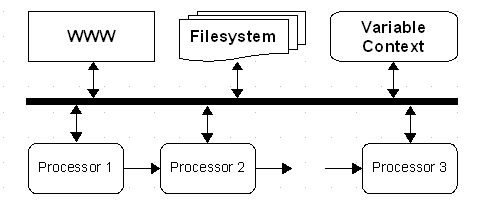
\includegraphics{./Figures/diagram1.png}
		\rule{35em}{0.5pt}
	\caption[Web-Harvest}
\end{figure}


The result of extraction could be available in files created during execution or from the variable context if Web-Harvest is programmatically used.
Configuration language

Every extraction process is defined in one or more configuration files, using simple XML-based language. Each processor is described by specific XML element or structure of XML elements. For the illustration, here is presented an example of configuration file:
you may check the XML configuration file here \ref{crawlersXML}

This configuration contains two pipelines. The first pipeline performs the following steps:
\begin{itemize}
\item [1] HTML content at http://news.bbc.co.uk is downloaded
\item [2] HTML cleaning is performed on downloaded content producing XHTML,
\item [3] XPath expression is searched for, giving URL sequence of page images,
\item [4] New variable named "urlList" is defined containing sequence of image URLs.
\end{itemize}
The second pipeline uses result of the previous execution in order to collect all page images:
\begin{itemize}
\item [1] Loop processor iterates over URL sequence and for every item:
\item [2] Downloads image at current URL,
\item [3] Stores the image on the file system.
\end{itemize}


\section{Corpus}
We used two corpora one of them is Al Jazeera, which contains 4462 article from various categories like Arts,culture,Economy, International, locals, Medical, Society, Sport.
The other corpus is upto-date corpus extracted using crawling tool with predefined XML files from specific News agency Like: Reuters, CNN, BBC, Al Arabiya, Youm7.This corpus was around 160 articles from many categories.



